\documentclass[12pt,a4paper]{scrartcl}
\usepackage[ngerman]{babel}
\usepackage[onehalfspacing]{setspace}

\usepackage[utf8]{inputenc}

\usepackage{graphicx,array,gnuplottex,siunitx,multicol,capt-of,amsmath,ulem,amsthm}
\let\phi\varphi

%---------------------------------------------------------------------------------------------------------------------------------------------------------------
% Ende der Einstellungen
%---------------------------------------------------------------------------------------------------------------------------------------------------------------

%---------------------------------------------------------------------------------------------------------------------------------------------------------------
%Ab hier gibt es Inhalt
%---------------------------------------------------------------------------------------------------------------------------------------------------------------
\begin{document}

\title{Heißluftmotor \\ (Korrektur)}
\author{Henrik Jäger \\ 3114168 \and Lena Majer \\ 3115808}
\subtitle{W40a \\  Assistent: Daniel Hirneise}
\subject{Physikalisches Praktikum I}
\publishers{Universität Stuttgart}
\date{\begin{tabular}{rr} Versuchstag: &15. Dezember 2016\\ 
Erste Abgabe: &22. Dezember 2016 \\
Abgabe Korrektur: &26. Januar 2017 \\ 
& 
\end{tabular}}
%\thanks{Assistent: Sascha Kolatschek}

\maketitle% Titelei
\pagebreak
\tableofcontents %Inhaltsverzeichnis
\pagebreak
\section{Einleitung}
\subsection{Ziel}
In diesem Versuch soll die abgeführte Wärmeenergie eines Prozesses (Heißluftmotor einmal als Kältemaschine und einmal als Wärmemaschine) in Abhängigkeit von der Zeit bestimmt werden. Zudem wird die Schmelzwärme von Wasser bestimmt.
\subsection{Grundlagen}
Der erste Satz der Thermodynamik ist gegeben durch:\\
\begin{equation}
\Delta U = \Delta Q + \Delta W
\end{equation}
Dieser Satz besagt, dass die innere Energie geändert werden kann, durch den Transport von Wärme oder Arbeit. Ist das System jedoch abgeschlossen, ist die Energie somit erhalten. Ein System verrichtet nur Arbeit, wenn von außen Wärme zugeführt wird.\\
Der zweite Hauptsatz der Thermodynamik besagt, Bei abgeschlossenen Systemen nimmt die Enthalpie zu, wenn der Prozess irreversibel ist. Die Enthalpie bleibt bei reversiblen Prozessen konstant. Wärme kann nie ganz in Arbeit umgewandelt werden.\\
Wenn man mit Gasen zu tun hat geht man häufig von idealen Gasen aus. Hierbei spielt das ideale Gasgesetz eine wichtige Rolle:\\
\begin{equation}
p \cdot V=n \cdot R\cdot T
\end{equation}
$P$ entspricht dem Druck in Pascal, $V$ entspricht dem Volumen in $m^3$, $n$ bezeichnet die Molzahl, $R$ ist die allgemeine Gaskonstante und $T$ entspricht der Temperatur in Kelvin.\\
Bei idealen Gasen kann zudem unterschieden werden um welche thermodynamische Prozesse es handelt. Unter einem isochoren Prozess versteht man ein gleichbleibendes Volumen. Dabei gilt:\\
\begin{equation}
\frac{P}{T}= const.
\end{equation}
 also
 \begin{equation}
 \frac{p_1}{T_1}= \frac{p_2}{T_2}
 \end{equation}
Bei gleichbleibendem Druck spricht man von einem isobaren Prozess. Hier gilt:\\
\begin{equation}
\frac{V}{T}= const.
\end{equation}
 also 
 \begin{equation}
  \frac{ V_1}{T_1}= \frac{V_2}{T_2}
 \end{equation}
Ein weiterer wichtiger Prozess ist der isotherme Prozess. Bei diesem Prozess ist die Temperatur konstant. Hier gilt:\\
\begin{equation}
p_1V_1 = p_2V_2
\end{equation}
Bei einer adiabatischen Zustandsänderung versteht man eine Zustandsänderung bei der gilt:
\begin{equation}
pV^\gamma = const.
\end{equation}
$\gamma$ kann experimentell bestimmt werden. Hierfür nimmt man eine Gasfeder zur Hilfe. \\
$\gamma$ kann auch durch spezifische Kapazitäten berechnet werden. Hierbei gilt:\\
\begin{equation}
\gamma =c_p/c_v
\end{equation}
 und \\
 \begin{equation}
 C_v = f/2 n R
 \end{equation}
 für konstantes Volumen\\
 \begin{equation}
 C_p = (f/2+1)n R
 \end{equation}
für konstanten Druck \\
Es gibt verschiedene Kreisprozesse. Bekannt ist der idealisierte Canot’sche Kreisprozess. Er besteht zwei Isothermen Zustandsänderungen und zwei Adiabaten Zustandsänderungen. \\
Im Vergleich besteht der Stirlingprozess aus Isothermen Zustandsänderungen und zwei Isochoren Zustandsänderungen.\\
Bei einem rechtsläufigen Prozess wird Thermische Energie in mechanische Arbeit umgewandelt. Handelt es sich dagegen um einen linksläufigen Prozesswird mit Hilfe von mechanischen Arbeit thermische Energie transportiert. Man spricht hierbei von einer Wärmepumpe.\\




\section{Messprinzip mit Skizze und Versuchsablauf} 
\subsection{Erster Versuchsteil}
Im ersten Versuchsteil wird mit einem linksdrehenden Stirlingmotor zunächst 1 cm$^3$ Wasser zum Gefrieren gebracht. Dabei wird die Drehzahl unter 200 Hz gehalten. Bei einer Temperatur von ca. -10 Grad Celsius wird gestoppt und die Maschine anders herum betrieben.
\subsection{Zweiter Versuchsteil}
Im zweiten Versuchsteil wird nun das gefrohrene Wasser aufgetaut und auf etwa 70 Grad Celsius erwärmt. Auch hierbei sollte die Drehzahl 200 Hz nicht überschreiten.
\subsection{Dritter Versuchsteil}
Im letzten Versuchsteil wird der Motor als rechtslaufender Kreisprozess verwendet. Nach einer Einschwingzeit wird zunächst die Leerlauffrequenz bestimmt. Anschließend wird ein Kreisprozess aufgenommen und die Fläche im $p$-$V$-Diagramm (entspricht der Arbeit) bestimmt. Zuletzt wird der Motor gebremst und dabei die verwendete Kraft und die daraus resultierende Frequenz bestimmt.
    
\pagebreak
\section{Messwerte}
Der Radius des Kolbens beträgt $0,0125\si{\metre}$\\
\\
Gemessene Werte: \\
\begin{center}
\begin{tabular}{c|c|c|c|c|c}
$f_0~[Hz]$ & $f_B~[Hz]$ & $F_1~[N]$ & $F_1~[N]$ & $\Delta F ~[N]$ & $P_B~[W]$\\ \hline \hline
219 & 2,15 & 7 & 4 & 3 & 0,058358225\\
196 & 3,266666667 & 14 & 4 & 10 & 0,295561037\\
166 & 2,766666667 & 19 & 6 & 13 & 0,325418733\\

\end{tabular}
\captionof{table}[]{Messwerte}
\end{center}
\begin{center}

\begin{gnuplot}[terminal=pdf,terminaloptions={font ",10" linewidth 1},scale=1.2]
		set xlabel "Zeit t [s]"
		set ylabel "Temperatur T [K]"
        set key left
   	 	set xrange [0:1400]
        set yrange [-10:70]
        
		plot 'Daten/data.csv' using 1:2 t "Temperatur" with lines
	\end{gnuplot}
    \captionof{figure}[DurchlassGerSil]{Messung der Temperatur der Wasserprobe} 
\end{center}

\pagebreak

\section{Formeln}
	Der ideale Wirkungsgrad ist:
\begin{align}
        	\eta_{id} = \frac{T_1 - T_3}{T_1}
        \end{align}
	Der effektive Wirkungsgrad beträgt dann:
        \begin{align}
        	\eta_{eff} = \frac{P_B}{P_e}
        \end{align}
        Für den inneren Wirkungsgrad:
        \begin{align}
        	\eta_{in} = \frac{P_{ind}}{P_e}
        \end{align}
        Und den mechanischen Wirkungsgrad:
        \begin{align}
        	\eta_{mech} = \frac{P_B}{P_{ind}}
        \end{align}
        Die entzogene Wärmemenge $ Q_s $ berechnet sich durch die Formel:
        \begin{equation}
         Q_s = P \cdot t_H
        \end{equation}
        Die Bremsleistung kann durch die Formel
        \begin{equation}
        P_B = 2\pi  F r f
        \end{equation}
        bestimmt werden.
        Die induzierte Leistung wird berechnet durch:
        \begin{equation}
        	P_{ind} = W_{ind} \cdot f 
        \end{equation}
        Dabei ist $W_{ind}$ die Fläche im pV-Diagramm.
\pagebreak

	\section{Auswertung}
     \begin{gnuplot}[terminal=pdf,terminaloptions={font ",10" linewidth 1},scale=1.2]
		set xlabel "Zeit t [s]"
		set ylabel "Temperatur T [K]"
        set key left
   	 	set xrange [0:1400]
        set yrange [-10:70]
        f(x)=-0.14*x+37.5
    	g(x)=0.3*(x-930)
        h(x)=10*(x-325)
        
		plot 'Daten/data.csv' using 1:2 t "Temperatur" with lines, f(x), g(x)
	\end{gnuplot}
    \captionof{figure}[DurchlassGerSil]{Messung der Temperatur der Wasserprobe} \ \\
    Um die Kühlleistung der Kältemaschine zu berechnen wird eine konstante Kühlleistung angenommen und die Steigung der Ausgleichsgeraden (In Abbildung 5.1 rot dargestellt) als  Quotient $\frac{\Delta T}{\Delta t}$ verwendet. Die Kühlleistung beträgt dann:
    \begin{align*}
    	P = \frac{\Delta Q}{\Delta t} = c\cdot m\cdot \frac{\Delta T}{ \Delta t} = 4128 \si{\joule\per\kilogram\kelvin} \cdot  10^{-3} \si{\kilogram} \cdot (-0,14) \si{\joule\per\second} = -0,5779 \si{\joule\per\second}
    \end{align*}
    Während des Gefriervorgangs muss die Kältemaschine dem Wasser weiter Energie entziehen, ohne dass sich die Temperatur ändert. Wenn die Kältemaschine auch weiterhin mit konstanter Leistung arbeitet, errechnet sich die entzogene Wärmemenge durch die Dauer dieses Vorgangs, der von $t_0 = 264,0 \si{\second}$ bis $t_1 = 602,2 \si{\second}$ andauert, wie folgt:
    \begin{align*}
    	 Q_s = P \cdot t_H = 0,5779 \si{\joule\per\second} \cdot (602,2 \si{\second} - 264,0 \si{\second}) = 195,4525 \si{\joule\per\gram}
    \end{align*}
    Der Literaturwert für Wasser ist $333,5 \si{\joule\per\gram}$. \\
    Die Erwärmung kann analog berechnet werden. Diesesmal wird für den Quotient $\frac{\Delta T}{\Delta t}$ die Steigung der grünen Ausgleichsgerade benutzt. Dabei wurde der Fit erst bei etwa $t = 1000s$ angelegt, da bis zu einer Temperatur von 20 Grad Celsius ein durch die Temperaturdifferenz ausgelöster rechtsläufiger Prozess entgegenwirkt.
    \begin{align*}
    	P = \frac{\Delta Q}{\Delta t} = c\cdot m\cdot \frac{\Delta T}{\Delta t} = 4128 \si{\joule\per\kilogram\kelvin} \cdot  10^{-3} \si{\kilogram} \cdot (0,3) \si{\joule\per\second} = 1,2384 \si{\joule\per\second}
    \end{align*}
    Die Schmelzwärme von Wasser ist betragsmäßig identisch mit seiner Kristallisationswärme und kann ebenfalls analog berechnet werden. Wie zuvor wird eine konstante Leistung angenommen.
    \begin{align*}
    	Q_s = P \cdot t_H = 1,2384 \si{\joule\per\second} \cdot (875,0 \si{\second} - 789,6 \si{\second}) = 205,7593 \si{\joule\per\gram}
    \end{align*}
    Die Werte stimmen nicht mit dem Literaturwert von $333,5 \si{\joule\per\gram}$ überein.
    
    \section{Wärmekraftmaschine}
    	Der Heizwendel wurde mit einer Leistung von 181 Watt betrieben, was nach dem im Versuchsraum ausliegendem Diagramm 840 Grad Celsius entspricht. Die Außentemperatur beträgt 26,6 Grad Celsius.
        Damit lässt sich der maximal mögliche Wirkungsgrad einer idealen Wärmekraftmaschine berechnen:
        \begin{align*}
        	\eta_{id} = \frac{T_1 - T_3}{T_1} = \frac{1113,15 \si{\kelvin} - 299,75 \si{\kelvin}}{1113,15 \si{\kelvin}} = 0,7307 = 73,07 \%
        \end{align*}
        Um die induzierte Leistung zu bestimmen, wurde die Fläche im p-V-Diagramm bestimmt und mit der Frequenz verrechnet.
        \begin{align*}
        P_{ind} = f \cdot W_{ind} = 2,15 \si{\hertz} \cdot 2,009 \si{\pascal\metre^3} = 4,4294 \si{\watt}
        \end{align*}
        Es wurden drei Bremsungen durchgeführt. beispielhaft für den ersten Wert berechnet sich die Bremsleistung mit:
        \begin{align*}
        	P_B = 2\pi  \Delta F r f = 2\pi \cdot 3 \si{\newton} \cdot 0,0125 \si{\metre} \cdot 2,15 \si{\hertz} = 0,5066 W
        \end{align*}
        Der effektive Wirkungsgrad beträgt dann 
        \begin{align*}
        	\eta_{eff} = \frac{P_B}{P_e} = \frac{0,5066 \si{\watt}}{181 \si{\watt}} = 0,0028 \rightarrow  0,28 \%
        \end{align*}
        Für den inneren Wirkungsgrad:
        \begin{align*}
        	\eta_{in} = \frac{P_{ind}}{P_e} = \frac{4,4294 \si{\watt}}{181 \si{\watt} } = 0,0245 \rightarrow  2,45\%
        \end{align*}
        Und den mechanischen Wirkungsgrad:
        \begin{align*}
        	\eta_{mech} = \frac{P_B}{P_{ind}} = \frac{0,5066 \si{\watt}}{4,294 \si{\watt}} = 0,1144 \rightarrow  11,44\%
        \end{align*}
        \begin{center}
        \begin{tabular}{c|cccccccc}
            Frequenz $f [\si{\hertz}]$ & Kraft $\Delta F [\si{\newton}]$& $P_{ind} [\si{\watt}]$ & $P_B [\si{\watt}]$	& $\eta_{eff}$	&$\eta_{in}$	&$\eta_{mech}$\\ \hline \hline
			2,15	&3	&4,3194	&0,5066	&0,0028	&0,0239	&0,1173\\
			3,27	&10	&6,5627	&2,5656	&0,0142	&0,0363	&0,3910\\
			2,77	&13	&5,5582	&2,8248	&0,0156	&0,0307	&0,5082\\ \hline
			&Mittelwerte&5,4801	&1,9657	&0,0109	&0,0303	&0,3388
        \end{tabular}
        \captionof{table}[]{Werte}
        \end{center}
        
        Der effektive Wirkungsgrad ist so viel niedriger als der ideale Wirkungsgrad, da kein idealer Stirling-Prozess abläuft. In Abbildung 5.2 wird deutlich, dass das p-V-Diagramm nicht wie ein Stirling-Prozess aussieht. \\
    	\begin{gnuplot}[terminal=pdf,terminaloptions={font ",10" linewidth 1},scale=1.2]
	
		set xlabel "Volumen V [ccm]"
		set ylabel "Druck p [hPa]"
        set key right
   	 	
		plot 'Daten/data2.csv' using 1:2 t "Wärmekraftmaschine" with lines
    
	\end{gnuplot}
    \captionof{figure}[DurchlassGerSil]{$p$-$V$ Diagramm der Wärmekraftmaschine} \ \\
	\pagebreak

	\section{Fehlerbetrachtung}
    	Im ersten Versuchsteil wurde zur Berechnung der Schmelzwärme angenommen, dass die Leistung der Wärmepumpe konstant ist. Außerdem wurde angenommen, dass das System isoliert ist, d.h. keine Wärme von außen das Wasser wieder erwärmt.
        Diese Annahmen können auch im zweiten Versuchsteil zu Fehlern führen. Im dritten Versuchsteil kann der Einschwingvorgang eventuell noch nicht beendet gewesen sein. Zudem ist das genaue Messen der Kräfte zusammen mit der momentanten Drehzahl sehr schwierig. Da sich der Kolben im reellen Fall nicht reibungsfrei bewegen kann, führt diese Reibung ebenfalls zu einem Fehler.
        
        Die Dichtheit des Kolbens spielt in allen Versuchsteilen eine Rolle.

\section{Zusammenfassung}
    Als Fehlerquellen dieses Versuchs spielen Ungenauigkeiten der Messgeräte wie dem Frequenzmesser oder dem Temperaturmesser eine Rolle. Ein weiteres Problem, ist das ,dass das System nicht ganz abgeschlossen ist. wärme kann nie ganz in das System zurückgeführt werden. Auch kann bei schwachen anschrauben der Schrauben des Glaszylinders Luft entweichen, was ebenfass zu Verfälschungen führen kann.\\
    \\
    aud diesem Versuch erhielt man, dass der rechtsläufige Motor einen effektiven Wirkungsgrad von $\eta_{eff} = 1,09 \%$  hat. Vergleicht man $ \eta_{id} = 73,07 \%$ mit $\eta_{eff} $, so sieht man, dass nur ein kleiner Teil der Energie in Arbeit umgewandelt wird. \\
    \\
    Aus der Kurve des linkslaufenden Prozesses abgelesen werden, dass die Leistung der Wärmepumpe $P_{Kuehl} = -1,73376 \si{\joule\per\second}$ für die Kühlung und $P_{Heiz} = 3,7152 \si{\joule\per\second}$ für die Heizung beträgt.
    
    Der Mittelwert der Schmelzwärme ist $<Q> = 200,6059 J$ stimmt nicht mit dem Literaturwert überein.
    Der Literaturwert für Wasser ist $333,5 \si{\joule\per\gram}$.

	\section{Anhang}
    	\begin{center}
    		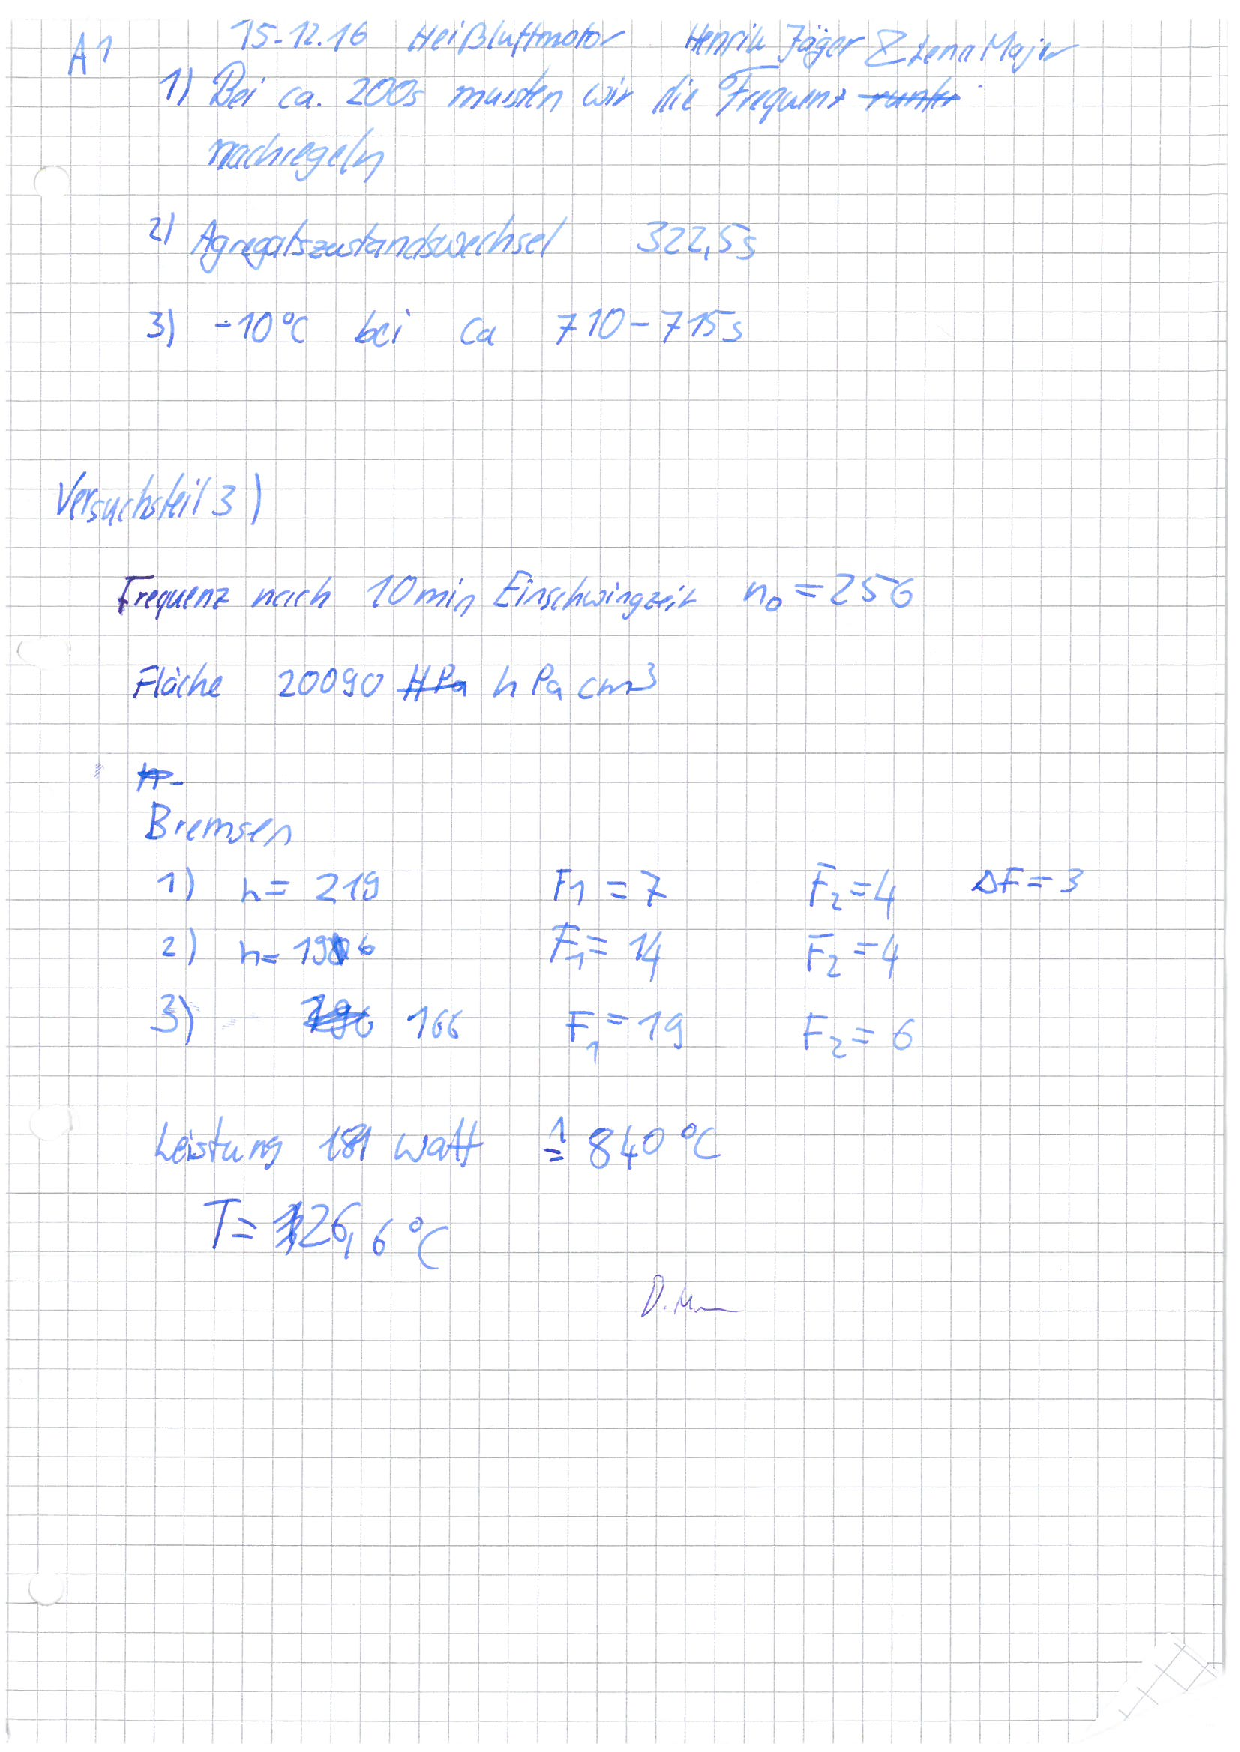
\includegraphics[scale=0.65]{1.pdf}
    	\end{center}
    	\captionof{figure}[Seite 1]{Messprotokoll}
	\pagebreak









\end{document}
